\documentclass[conference]{IEEEtran}
\IEEEoverridecommandlockouts
% The preceding line is only needed to identify funding in the first footnote. If that is unneeded, please comment it out.
\usepackage{cite}
\usepackage{amsmath,amssymb,amsfonts}
\usepackage{algorithmic}
\usepackage{graphicx}
\usepackage{dblfloatfix}

\def\BibTeX{{\rm B\kern-.05em{\sc i\kern-.025em b}\kern-.08em
    T\kern-.1667em\lower.7ex\hbox{E}\kern-.125emX}}
\begin{document}

\title{Bayesian learning of finite Asymmetric Gaussian mixtures with MH-within-Gibbs method\\
%{\footnotesize \textsuperscript{*}Note: Sub-titles are not captured in Xplore and
%should not be used}
%\thanks{Identify applicable funding agency here. If none, delete this.}
}

\author{\IEEEauthorblockN{1\textsuperscript{st} Shuai Fu}
\IEEEauthorblockA{\textit{Faculty of Engineering and Computer Science}\\
\textit{Concordia University}\\
Montreal, Canada\\
f\_shuai@encs.concordia.ca}
\and
\IEEEauthorblockN{2\textsuperscript{nd} Nizar Bouguila}
\IEEEauthorblockA{\textit{Concordia Institute for Information Systems Engineering} \\
\textit{Concordia University}\\
Montreal, Canada \\
bouguila@ciise.concordia.ca}
}

\maketitle

\begin{abstract}
Asymmetric Gaussian mixture (AGM) model has been proved more flexible than the classic symmetric Gaussian mixture model because no constrain will be given that the distribution of observations should be symmetric from the proposed mean of every dimension. This paper introduces a fully Bayesian learning method using Metropolis-Hastings within Gibbs sampling method and its applications.
\end{abstract}

\begin{IEEEkeywords}
Asymmetric Gaussian mixture, AGM, Asymmetric Gaussian distribution, AGD, Metropolis-Hastings method, Gibbs sampling, Markov chain Monte Carlo, MCMC, MH-within-Gibbs, Bayesian analysis
\end{IEEEkeywords}

\section{Introduction}
This paper is trying to introduce a new Bayesian model which combines AGM model (Elguebaly and Bouguila, 2013) \cite{b1} with random sampling based Markov chain Monte Carlo (MCMC) method for mixture parameter learning. Distinguished to traditional expectation-maximization (Wu, 1983)\cite{b2} learning method, sampling-based Markov chain Monte Carlo method considers not only posterior distribution (likelihood) but also involves proposed prior and posterior distributions for every mixture parameter which is not deterministic and brings randomness into the learning procedure. As a variation of classic MCMC method, the Metropolis-Hastings-within-Gibbs sampling method (Bouguila, Ziou and Hammoud, 2008)\cite{b3} takes the advantages of both Gibbs sampling and Metropolis-Hastings method while sampling from proposed distributions of mixture parameters could be flexible and adjustable depending on specific applications and datasets. 

Compared to classic Gaussian distribution, the mean of asymmetric Gaussian distribution (AGD) is as the same as symmetric one, however, AGD is using two independent standard deviation vectors to define 'left' and 'right' parts of the model. Therefore, AGD can be seen as a combination of multiple symmetric Gaussian distributions depending on the dimension \textsl{d} thus it can be easily extended as a multi-dimensional model.

Monte Carlo method is well known as an effective random sampling method for estimation purpose and Markov chain defines rules how model transfers from one to another. Based on the characteristics of the AGM model, MCMC method is selected to be the learning algorithm for the estimation of mixture parameters.In fact,Metropolis-Hastings method (Hastings, 1970)\cite{b4} and Gibbs sampling (Geman and Geman, 1984)\cite{b5} are two most widely used implementations of MCMC method.Although the acceptance ratio of Gibbs sampling is always be 1 means every move will be accepted, when direct sampling from the distribution is not easy, Metropolis-Hastings method provides an alternative.

According to the organization of this paper, Section 2 will be the illustration of AGM model and Bayesian learning processes. In Section 3, both experimental and real applications will be applied to the mixture model and the results will be analyzed.


\section{Bayesian model}
\subsection{Asymmetric Gaussian mixture model}
Assuming that the AGM model has \textsl{M} components and the likelihood function (Elguebaly and Bouguila, 2013)\cite{b1} is defined as follows:
\begin{align}
P(\chi|\Theta) = \prod_{i=i}^N \sum_{j=1}^Mp_jP(X_i|\xi_j)
\label{eq:1}
\end{align}
where $\chi = (X_1,...,X_N)$ is the set of observations with total amount of $N$, $\Theta = \{p_1,...,p_M, \xi_1,...,\xi_M\}$ represents the parameter sets of M mixture components for the AGM model, $p_j$ (0 $< p_j \leq$ 1 and $\sum_{j=1}^Mp_j$ = 1) is the weight for each component in the mixture model and $\xi_j$ is the AGD parameters of mixture component j.

In order to simplify the Bayesian learning process, we introduced the membership vector $Z_i=(Z_{i1},...,Z_{iM})$. For each observation $X_i, 1 < i <N, Z_i = (Z_{i1},...,Z_{iM})$ is a M-dimensional membership vector which indicates $X_i$ belongs to a specific component (Bouguila, Ziou and Monga, 2006)\cite{b6}, such that:
\begin{align}
Z_{ij} = \left\{\begin{matrix}
1\ \qquad if\ X_i\ belongs\ to\ component\ j \\
0\ \qquad\quad\qquad otherwise\qquad\qquad\quad\quad \\
\end{matrix}\right.
\label{eq:2}
\end{align}
in another word, $Z_{ij} = 1$ only if observation $X_i$ has the highest probability of belonging to component j and accordingly, for other components, $Z_{ij} = 0$. 

Combine the Eq. \eqref{eq:1} and Eq. \eqref{eq:2} together we derived the new density function:
\begin{align}
P(\chi, Z|\Theta) = \prod_{i=1}^{N}\prod_{j=1}^{M}(p_jP(X_i|\xi_j))^{Z_{ij}}
\label{eq:3}
\end{align}

Specifically for AGM model, concerning observation X belongs to mixture component j and $X = (x_1,...,x_d)$, the probability density function (Elguebaly and Bouguila, 2013)\cite{b1} can be defined as following:
\begin{multline}
P(X|\xi_j) \propto \prod_{k=1}^{d} \frac{1}{(\sigma_{l_{jk}}+\sigma_{r_{jk}})}\\
\times \left\{\begin{matrix}
\exp \begin{bmatrix}
-\frac{(x_k-\mu_{jk})^2}{2(\sigma_{l_{jk}})^2}
\end{bmatrix}\ if\ x_k\ <\ \mu_{jk} \\ 
\exp \begin{bmatrix}
-\frac{(x_k-\mu_{jk})^2}{2(\sigma_{r_{jk}})^2}
\end{bmatrix}\ if\ x_k\ \geqslant\ \mu_{jk} \\ 
\end{matrix}\right.
\label{eq:4}
\end{multline}
where $\xi_j = (\mu_j,\sigma_{lj},\sigma_{rj})$ is the set of parameters of component j and $\mu_j = (\mu_{j1},...,\mu_{jd})$ is the mean, $\sigma_{lj} = (\sigma_{lj1},...,\sigma_{ljd})$ and $\sigma_{rj} = (\sigma_{rj1},...,\sigma_{rjd})$ are the left and right standard deviations for AGD. To be more specific, $x_k \thicksim N(\mu_{jk},\sigma_{ljk})\ (x_k < \mu_{jk})$ and $x_k \thicksim N(\mu_{jk},\sigma_{rjk})\ (x_k \geqslant \mu_{jk})$ for each dimension.

\subsection{Learning algorithm}
Before describing detailed MH-within-Gibbs learning steps, some priors and posteriors need to be clarified that having the membership vector in hand,  we denote the postorior probability of membership vector Z as $\pi(Z|\Theta,\chi)$ (Elguebaly and Bouguila, 2011)\cite{b7}. Therefore, during the iteration $t$ of learning process:
\begin{align}
Z^{(t)} \sim \pi(Z|\Theta^{(t-1)},\chi)
\label{eq:5}
\end{align}
then derive the number of observations belonging to a specific component j according to $Z^{(t)}$ as follows:
\begin{align}
n_j^{(t)} = \sum_{i=1}^NZ_{ij}\ (j = 1,...,M) 
\label{eq:6}
\end{align}
thus $n^{(t)}=(n_i^{(t)},...,n_M^{(t)})$ represents the number of observations belonging to each mixture component.

Since the mixture weight $p_j$ (0 $< p_j \leq$ 1 and $\sum_{j=1}^Mp_j$ = 1), a nature choice of the prior is Dirichlet distribution as following (Marin, Mengersen and Robert, 2005) \cite{b8}: 
\begin{align}
\pi(p_j^{(t)}) \sim \textit{D}(\gamma_1,...,\gamma_M )
\label{eq:7}
\end{align}
where $\gamma_j)$ is known hyperparameter. Consequently, the posterior of the mixture weight $p_j$ is:
\begin{align}
P(p_j^{(t)}|Z^{(t)}) \sim \textit{D}(\gamma_1 + n_1^{(t)},...,\gamma_M + n_M^{(t)})
\label{eq:8}
\end{align}


As mentioned before, direct sampling of mixture parameters $\xi \sim P(\xi|Z,\chi)$ could be difficult so Metropolis-Hastings method should be involved to propose proposal distributions for $\xi^{(t)} \sim q(\xi|\xi^{(t-1)})$. To be more specific, for parameters of AGM model which are $\mu$ , $\sigma_l$ and $\sigma_r$, we choose proposal distributions as follows:
\begin{align}
\mu_j^{(t)} \sim \textit{N}_d(\mu_j^{(t-1)},\Sigma)
\label{eq:9}
\end{align}
\begin{align}
\sigma_{lj}^{(t)} \sim \textit{N}_d(\sigma_{lj}^{(t-1)},\Sigma)
\label{eq:10}
\end{align}
\begin{align}
\sigma_{rj}^{(t)} \sim \textit{N}_d(\sigma_{rj}^{(t-1)},\Sigma)
\label{eq:11}
\end{align}
the proposal distributions are $d$-dimensional Gaussian distributions with $\Sigma$ as $d$ x $d$ identity matrices which make the sampling as random walk MCMC process.

As the most important part of Metropolis-Hastings method, at the end of each iteration, for new generated mixture parameter set $\Theta^{(t)}$, an acceptance ratio $r$ needs to be calculated in order to make a decision whether they should be accepted or discarded for the next iteration. For acceptance ration $r$, compute:
\begin{align}
r = \frac{P(\chi|\Theta^{(t)})\pi(\Theta^{(t)})q(\Theta^{(t-1)}|\Theta^{(t)})}{P(\chi|\Theta^{(t-1)})\pi(\Theta^{(t-1)})q(\Theta^{(t)}|\Theta^{(t-1)})}
\label{eq:12}
\end{align}

where $\pi(\Theta)$ is the proposed prior distribution which can be decomposed to $d$-dimensional Gaussian distributions that $\mu \sim \textit{N}_d(\eta,\Sigma)$ and $\sigma_l, \sigma_r \sim \textit{N}_d(\tau,\Sigma)$ given known hyperparameters $\eta$ and $\tau$. Since mixture weight $p$ has been computed previously during the Gibbs sampling part, it should not be included in Eq. \eqref{eq:12}. Further information about the calculation of acceptance ratio $r$ is explained in Appendix A.

Once acceptance ratio $r$ is derived by Eq. \eqref{eq:15}, compute acceptance probability $\alpha = min[1,r]$ (Luengo, D. and Martino, L., 2013) \cite{b9}. Then $u \sim U_{[0,1]}$ is supposed to be generated randomly. If $\alpha < u$, the proposed move should be accepted and parameters should be updated by $p^{(t)}$ and $\xi^{(t)}$ for next iteration. Otherwise, discard $p^{(t)}$, $\xi^{(t)}$ and set $p^{(t)} = p^{(t-1)}$, $\xi^{(t)} = \xi^{(t-1)}$.

We summarize the MH-within-Gibbs learning process for AGM model as the following steps:
\bigbreak
\noindent\textbf{Input:} Data observations $\chi$ and component number M \\
\textbf{Output:} AGM mixture parameter set $\Theta$
\bigbreak

\begin{enumerate}
\item Initialization
\item Step $t$: For $t = 1,\ldots$
\begin{enumerate}
\item[]\textbf{Gibbs part}
\item Generate $Z^{(t)}$ from Eq. \eqref{eq:5}
\item Compute $n_j^{(t)}$ from Eq. \eqref{eq:6}
\item Generate $p_j^{(t)}$ from Eq. \eqref{eq:8}
\item[] \textbf{Metropolis-Hastings part}
\item Sample $\xi_j^{(t)}$ ($\mu_j^{(t)}, \sigma_{lj}^{(t)}, \sigma_{rj}^{(t)}$) from Eqs. \eqref{eq:9} \eqref{eq:10} \eqref{eq:11}
\item Compute acceptance ratio $r$ from Eq. \eqref{eq:15}
\item Generate $\alpha = min[1,r]$ and $u \sim U_{[0,1]}$
\item If $\alpha \geq u$ then $\xi^{(t)} = \xi^{(t-1)}$
\end{enumerate}
\end{enumerate}


\begin{figure*}[b]
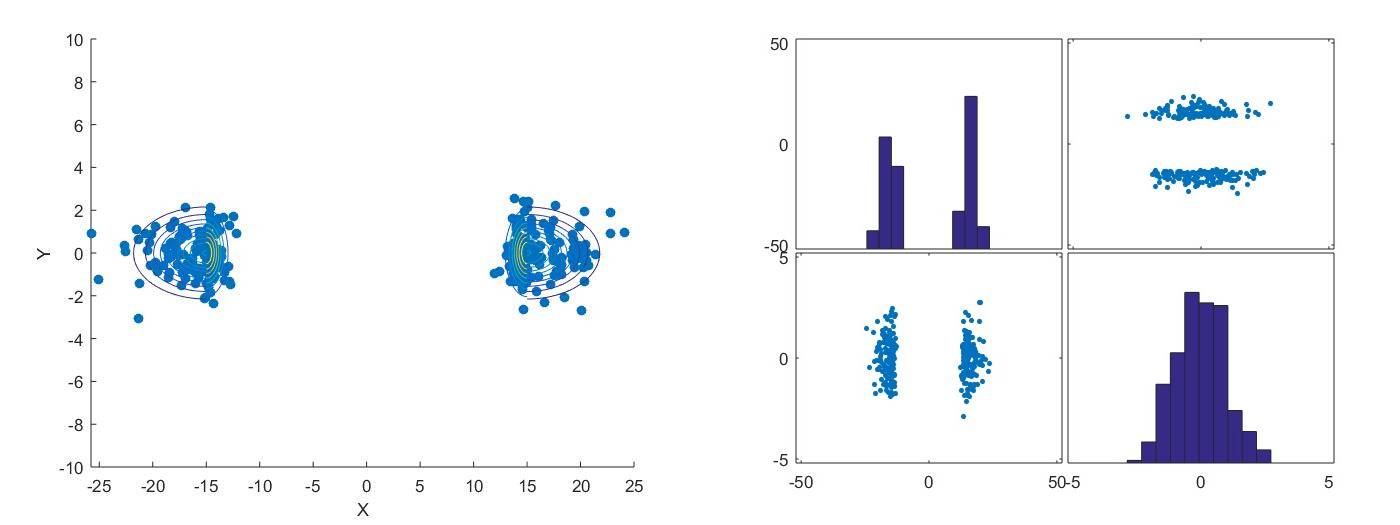
\includegraphics[height=0.3\textheight]{12.jpg}
\caption{Original synthetic observations}
\label{fig:1}
\end{figure*}

\begin{figure*}[b]
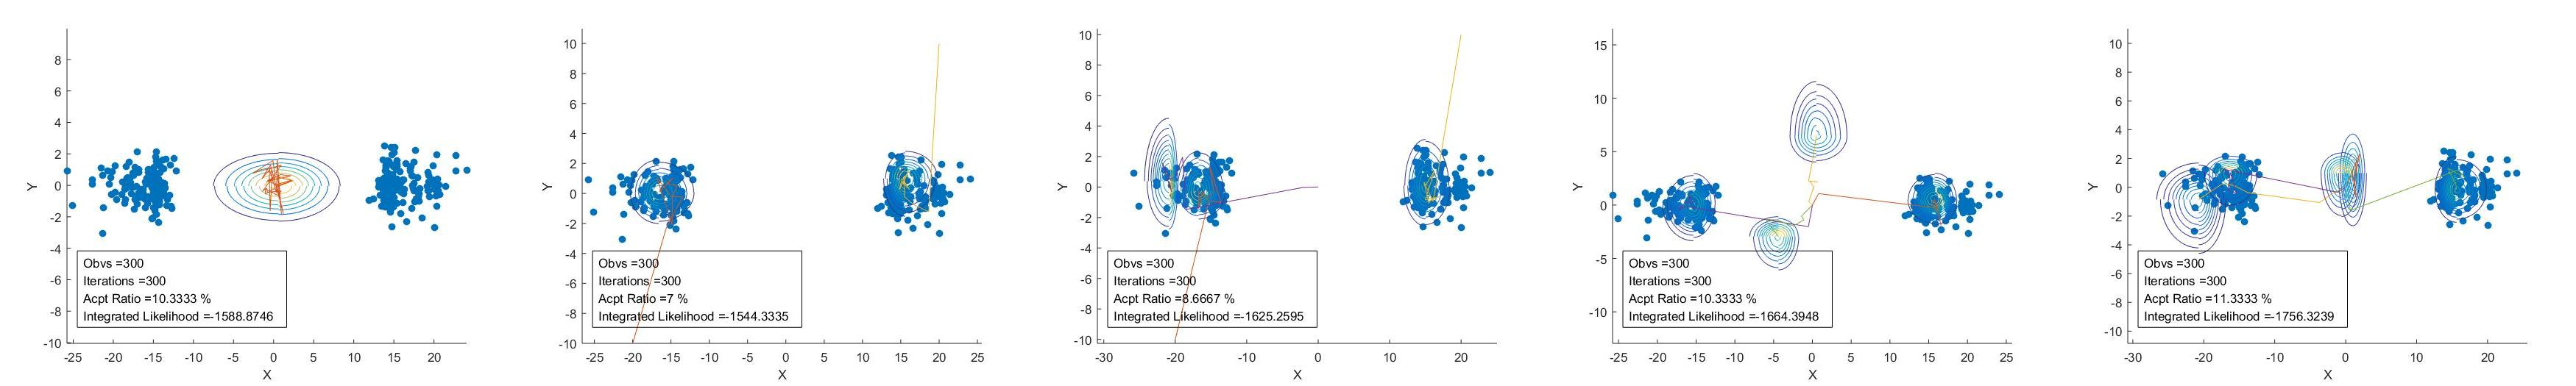
\includegraphics[height=0.12\textheight]{23456.jpg}
\caption{AGM learning results (proposed component number $k = 1,\dots,5$, iteration = 300)}
\label{fig:2}
\end{figure*}

\section{Experimental results}
\subsection{Design of experiments}
We apply the AGM model to both synthetic data and intrusion detection application. For synthetic data validation part, testing observations will be generated from AGD with known component number $M$. NSL-KDD dataset (Tavallaee, M., Bagheri, E., Lu, W. and Ghorbani, A.A., 2009) \cite{b10} is selected for intrusion detection part.

\subsection{Synthetic data}
The main goals of this section are feasibility analysis and evaluating the efficiency of the AGM learning algorithm.

Observation number is set to 300 spliting into two groups. Fig. \ref{fig:1} displayed observation distribution and its histograms for both dimensions. Hyperparameters are set accordingly as $\gamma_j$ introduced in Eq. \eqref{eq:7} is 1 (Stephens, M., 2000) \cite{b11} for sampling of proposed mixture weight $p_j$, $\eta$ and $\tau$ are $d$-dimensional zero vectors for prior distributions of mixture parameter $\xi$.

Probability density diagrams with different component values of $k\ (k = 1,\dots,5)$ are shown in Fig. \ref{fig:2}. Polylines ploted the trace of accepted moves of each component. Obviously, the best result is derived when component number $k$ equals to 2 which is the same as the number of observation groups. Furthermore, it has the maximum marginal likelihood value which also indicates the best component number.

AGM learning statistics summarized in Table \ref{tab1} shows that the algorithm leads to the convergence within 300 iterations and accepted moves are less than 35. From the best test result ($k$ = 2), algorithm was converged after 21 accepted moves without abnormal shaking and drifting.

\begin{table}[b]
\caption{AGM learning statistics}
\begin{center}
\begin{tabular}{|c|c|c|c|}
\hline
\textbf{Comp. Num. $k$} & \textbf{\textit{Moves Accepted}}& \textbf{\textit{Acceptance Ratio}}& \textbf{\textit{ML$^{\mathrm{a}}$}} \\
\hline
1 & 31 & -1588.8746 & 10.3\%  \\
2 & 21 & -1544.3335 & 7.0\% \\
3 & 26 & -1625.2595 & 8.7\% \\
4 & 31 & -1664.3948 & 10.3\% \\
5 & 34 & -1756.3239 & 11.3\% \\
\hline
\multicolumn{4}{l}{$^{\mathrm{a}}$Marginal likelihood.}
\end{tabular}
\label{tab1}
\end{center}
\end{table}

\subsection{Intrusion detection (TBD)}
TBD

\section{Conclusion (TBD)}
TBD

\section*{Acknowledgment (TBD)}
TBD

\section*{Appendix A}
\subsection{Derivation of acceptance ratio $r$ by Eq. \eqref{eq:12}}
The derivation of acceptance ratio $r$ is based on the assumption that mixture parameters are independent from each other which means that:
\begin{multline}
\pi(\Theta) = \pi(p,\xi) = \pi(\xi) \\
= \prod_{j=1}^M\pi(\mu_j)\pi(\sigma_{lj})\pi(\sigma_{rj})\qquad\qquad\qquad\qquad \\
= \prod_{j=1}^M\textit{N}_d(\mu_j|\eta,\Sigma)\textit{N}_d(\sigma_{lj}|\tau,\Sigma)\textit{N}_d(\sigma_{rj}|\tau,\Sigma)\quad
\label{eq:13}
\end{multline}
in Eq. \eqref{eq:14}, since the mixture weigh $p$ is generated following Gibbs sampling method which acceptance ratio is always 1, it should be excluded from Metropolis-Hastings estimation step. Accordingly, apply the same rule to the proposal distribution as well:
\begin{multline}
q(\Theta^{(t)}|\Theta^{(t-1)}) = q(\xi^{(t)}|\xi^{(t-1)}) \\
= \prod_{j=1}^M\textit{N}_d(\mu_j^{(t)}|\mu_j^{(t-1)},\Sigma)\textit{N}_d(\sigma_{lj}^{(t)}|\sigma_{lj}^{(t-1)},\Sigma)\textit{N}_d(\sigma_{rj}^{(t)}|\sigma_{rj}^{(t-1)},\Sigma)
\label{eq:14}
\end{multline}
combines Eqs. \eqref{eq:1} \eqref{eq:4} \eqref{eq:9} \eqref{eq:10} \eqref{eq:11} \eqref{eq:14} and \eqref{eq:15}, equation \eqref{eq:12} can be written as follows:

\begin{multline}
r = \frac{P(\chi|\Theta^{(t)})\pi(\Theta^{(t)})q(\Theta^{(t-1)}|\Theta^{(t)})}{P(\chi|\Theta^{(t-1)})\pi(\Theta^{(t-1)})q(\Theta^{(t)}|\Theta^{(t-1)})} \\
= \prod_{i=i}^N \prod_{j=1}^M(\frac{P(X_i|\mu_j^{(t)},\sigma_{lj}^{(t)},\sigma_{rj}^{(t)})}
{P(X_i|\mu_j^{(t-1)},\sigma_{lj}^{(t-1)},\sigma_{rj}^{(t-1)})} \qquad\qquad\quad \\
\times \frac{\textit{N}_d(\mu_j^{(t)}|\eta,\Sigma)\textit{N}_d(\sigma_{lj}^{(t)}|\tau,\Sigma)\textit{N}_d(\sigma_{rj}^{(t)}|\tau,\Sigma)}{\textit{N}_d(\mu_j^{(t-1)}|\eta,\Sigma)\textit{N}_d(\sigma_{lj}^{(t-1)}|\tau,\Sigma)\textit{N}_d(\sigma_{rj}^{(t-1)}|\tau,\Sigma)} \\
\times \scalebox{1.01}{$\frac{\textit{N}_d(\mu_j^{(t-1)}|\mu_j^{(t)},\Sigma)\textit{N}_d(\sigma_{lj}^{(t-1)}|\sigma_{lj}^{(t)},\Sigma)\textit{N}_d(\sigma_{rj}^{(t-1)}|\sigma_{rj}^{(t)},\Sigma)}{\textit{N}_d(\mu_j^{(t)}|\mu_j^{(t-1)},\Sigma)\textit{N}_d(\sigma_{lj}^{(t)}|\sigma_{lj}^{(t-1)},\Sigma)\textit{N}_d(\sigma_{rj}^{(t)}|\sigma_{rj}^{(t-1)},\Sigma)}$})
\label{eq:15}
\end{multline}

\begin{thebibliography}{00}
\bibitem{b1} Elguebaly, T. and Bouguila, N. (2013). Background subtraction using finite mixtures of asymmetric Gaussian distributions and shadow detection. Machine Vision and Applications, 25(5), pp.1145-1162.
\bibitem{b2} Wu, C. (1983). On the Convergence Properties of the EM Algorithm. The Annals of Statistics, 11(1), pp.95-103.
\bibitem{b3} Bouguila, N., Ziou, D. and Hammoud, R. (2008). On Bayesian analysis of a finite generalized Dirichlet mixture via a Metropolis-within-Gibbs sampling. Pattern Analysis and Applications, 12(2), pp.151-166.
\bibitem{b4} Hastings, W. (1970). Monte Carlo Sampling Methods Using Markov Chains and Their Applications. Biometrika, 57(1), p.97.
\bibitem{b5}Geman, S. and Geman, D. (1984). Stochastic Relaxation, Gibbs Distributions, and the Bayesian Restoration of Images. IEEE Transactions on Pattern Analysis and Machine Intelligence, PAMI-6(6), pp.721-741.
\bibitem{b6} Bouguila, N., Ziou, D. and Monga, E. (2006). Practical Bayesian estimation of a finite beta mixture through gibbs sampling and its applications. Statistics and Computing, 16(2), pp.215-225.
\bibitem{b7} Elguebaly, T. and Bouguila, N. (2011). Bayesian learning of finite generalized Gaussian mixture models on images. Signal Processing, 91(4), pp.801-820.
\bibitem{b8} Marin, J.M. and Mengersen, K.R.C., 2005. Handbook of Statistics: Bayesian modelling and inference on mixtures of distributions, Vol. 25.
\bibitem{b9} Luengo, D. and Martino, L., 2013, May. Fully adaptive gaussian mixture metropolis-hastings algorithm. In Acoustics, Speech and Signal Processing (ICASSP), 2013 IEEE International Conference on (pp. 6148-6152). IEEE.
\bibitem{b10} Tavallaee, M., Bagheri, E., Lu, W. and Ghorbani, A.A., 2009, July. A detailed analysis of the KDD CUP 99 data set. In Computational Intelligence for Security and Defense Applications, 2009. CISDA 2009. IEEE Symposium on (pp. 1-6). IEEE.
Vancouver	
\bibitem{b11} Stephens, M., 2000. Bayesian analysis of mixture models with an unknown number of components-an alternative to reversible jump methods. Annals of statistics, pp.40-74.
\end{thebibliography}

\end{document}
